% Компіляція: lualatex -shell-escape main.tex (двічі)
\documentclass[12pt,a4paper]{article}

\usepackage{fontspec}
\usepackage{polyglossia}
\setdefaultlanguage{ukrainian}
\setmainfont{NewComputerModern10}
\setsansfont{Noto Sans}
\setmonofont{Noto Sans Mono}[Scale=0.82,ItalicFont={Noto Sans Mono},ItalicFeatures={FakeSlant=0.2}]

\usepackage{amsmath,amssymb,array,booktabs,caption,enumitem,float,geometry,graphicx,microtype,titlesec,xcolor}
\geometry{left=2cm,right=2cm,top=2cm,bottom=2cm}
\setlength{\parindent}{1.25cm}
\setlength{\parskip}{0pt}
\linespread{1.08}
\titleformat{\section}{\normalfont\fontsize{14}{16}\selectfont\bfseries}{\thesection}{0.6em}{}
\titleformat{\subsection}{\normalfont\fontsize{12}{14}\selectfont\bfseries}{\thesubsection}{0.6em}{}
\titlespacing*{\section}{0pt}{1.4em}{0.65em}
\titlespacing*{\subsection}{0pt}{1.1em}{0.45em}
\captionsetup{font=small,labelfont=bf,labelsep=endash}
\captionsetup[table]{position=bottom,skip=5pt}

\usepackage[newfloat]{minted}
\SetupFloatingEnvironment{listing}{name=Лістинг}
\setminted{fontsize=\scriptsize,linenos,breaklines,breakanywhere,autogobble,frame=single,framesep=2mm,bgcolor=gray!5,tabsize=4}

\usepackage[unicode,colorlinks=true,linkcolor=black,urlcolor=blue,
  pdftitle={ІО-41, Давидчук Артем, Вступ до штучного інтелекту, Лабораторна робота №2},
  pdfauthor={Давидчук Артем},
  pdfsubject={Інтелектуальні агенти}]{hyperref}

\begin{document}

\pagenumbering{gobble}
\begin{titlepage}
  \begin{center}
    
\includegraphics[width=0.7\textwidth]{../../../../../../templates/letterhead.png}
  \end{center}

  \begin{center}
    \large
    Національний технічний університет України\\
    «Київський політехнічний інститут імені Ігоря Сікорського»\\[1em]
    Факультет інформатики та обчислювальної техніки\\
    Кафедра обчислювальної техніки
  \end{center}

  \vfill
  \begin{center}
    \textbf{\LARGE Вступ до штучного інтелекту}\\[2em]
    \textbf{\Large Лабораторна робота №2}\\[0.7em]
    \parbox{0.9\textwidth}{\centering «Інтелектуальні агенти»}
  \end{center}

  \vfill
  \begin{flushright}
    \begin{minipage}{0.48\textwidth}
      Виконав: студент групи ІО-41\\
      \textit{Давидчук Артем}\\[1em]
      Перевірив: \textit{Кочура Ю. П.}
    \end{minipage}
  \end{flushright}

  \vfill
  \begin{center}Київ --- 2026\end{center}
\end{titlepage}
\pagenumbering{arabic}

\section{Мета роботи}

Розробити раціонального інтелектуального агента --- мережевого контролера,
який прокладає шлях від вузла-відправника до вузла-отримувача у зваженому
графі-топології мережі. Дослідити роботу агента з обмеженою видимістю та
порівняти знайдений ним маршрут з оптимальним маршрутом, отриманим за
алгоритмом Дейкстри.

\section{Постановка задачі}

Для виконання роботи використано граф із лабораторної роботи №1. Вершини
графа відповідають мережевим вузлам, ребра --- каналам зв'язку, а вага ребра
моделює затримку передавання даних у мілісекундах.

Контролер отримує адреси початкового та кінцевого вузлів і повинен побудувати
між ними маршрут. На кожному кроці агент бачить тільки поточний вузол, його
безпосередніх сусідів і ваги відповідних каналів. Якщо обраний напрямок
приводить у тупик, агент відкликає останнє правило пересилання та повертається
до попереднього вузла.

\section{Теоретичні відомості}

\subsection{Інтелектуальний агент}

Інтелектуальний агент --- це система, яка сприймає стан середовища, вибирає
дію та виконує її для досягнення певної мети. У цій роботі відповідності між
складовими агента мають вигляд:

\begin{table}[H]
\centering
\begin{tabular}{>{\raggedright\arraybackslash}p{0.35\textwidth} p{0.52\textwidth}}
\toprule
\textbf{Складова} & \textbf{Реалізація у роботі}\\
\midrule
Середовище & зважений граф комп'ютерної мережі\\
Сприйняття & поточний вузол, сусіди та ваги каналів\\
Дії & встановлення або відкликання правила пересилання\\
Мета & досягнення вузла-отримувача\\
Показник ефективності & сумарна затримка маршруту\\
\bottomrule
\end{tabular}
\caption{Відповідність понять інтелектуального агента}
\end{table}

Раціональний агент обирає дію, яка, з урахуванням доступної інформації,
найкраще наближає його до мети. Через обмежену видимість такий агент не
гарантує глобально найкоротший шлях.

\subsection{Пошук із поверненням}

У роботі використано пошук із поверненням назад. Для поточного вузла агент
формує список невідвіданих сусідів та впорядковує його за вагою ребра:

\begin{equation}
  v^* = \arg\min_{v\in N(u)\setminus V_{visited}} w(u,v),
\end{equation}

де (N(u)) --- множина сусідів поточного вузла (u), а (w(u,v)) --- вага
ребра. Якщо невідвіданих сусідів немає, агент відкликає останнє правило,
видаляє вузол із поточного маршруту та повертається на попередню позицію.

\subsection{Алгоритм Дейкстри}

Алгоритм Дейкстри знаходить найкоротші шляхи у графі з невід'ємними вагами.
На початку початковій вершині призначається відстань нуль, а всім іншим ---
нескінченність. Потім обирається невідвідана вершина з найменшою відомою
відстанню та оновлюються відстані до її сусідів. Алгоритм використовує повну
топологію графа, тому його результат є еталонним для порівняння.

Для маршруту $P=(v_0,v_1,\ldots,v_k)$ сумарна затримка обчислюється так:

\begin{equation}
  D(P)=\sum_{i=0}^{k-1}w(v_i,v_{i+1}).
\end{equation}

\section{Опис програмної реалізації}

Генерація графа виконується функціями з модуля \texttt{lab1.py}. Основні
функції агента визначені безпосередньо в notebook \texttt{lab2.ipynb}.

\subsection{Вибір наступного вузла}

Сусіди поточного вузла сортуються за вагою ребра, а відвідані вузли
виключаються, щоб агент не потрапляв у цикли.

\begin{listing}[H]
\begin{minted}{python}
candidates = sorted(
    (
        (neighbor, edge_weight(graph, current, neighbor))
        for neighbor in graph.neighbors(current)
        if neighbor not in visited
    ),
    key=lambda item: item[1],
)
\end{minted}
\caption{Формування впорядкованого списку локальних варіантів}
\end{listing}

\subsection{Пошук агента}

Рекурсивна функція \texttt{search} перевіряє досягнення цілі, переходить до
невідвіданого сусіда та при невдалому переході виконує повернення назад.

\begin{listing}[H]
\begin{minted}{python}
def search(current):
    if current == target:
        return True

    for neighbor, weight in candidates:
        visited.add(neighbor)
        path.append(neighbor)
        installed_rules += 1

        if search(neighbor):
            return True

        path.pop()
        revoked_rules += 1

    return False
\end{minted}
\caption{Основна логіка пошуку з поверненням}
\end{listing}

\subsection{Порівняння з Дейкстрою}

Для еталонного маршруту використано реалізацію з бібліотеки NetworkX:

\begin{listing}[H]
\begin{minted}{python}
def dijkstra_path(graph, start, target):
    return nx.shortest_path(
        graph,
        start,
        target,
        weight="weight",
    )
\end{minted}
\caption{Пошук оптимального маршруту за Дейкстрою}
\end{listing}

\section{Результати роботи}

Для першого експерименту використано граф із 25 вузлів, 6 видаленими ребрами
та вагами каналів від 1 до 10. Початковий вузол --- \texttt{(0, 0)}, кінцевий
вузол --- \texttt{(4, 4)}. Для відтворення результатів використано фіксоване
початкове значення генератора випадкових чисел \texttt{42}.

Агент побудував маршрут із 17 вузлів. Сумарна затримка маршруту агента
становить 51 мс, а алгоритм Дейкстри знайшов маршрут із затримкою 31 мс.
Під час пошуку агент встановив 18 правил і відкликав 2 правила.

\begin{figure}[H]
  \centering
  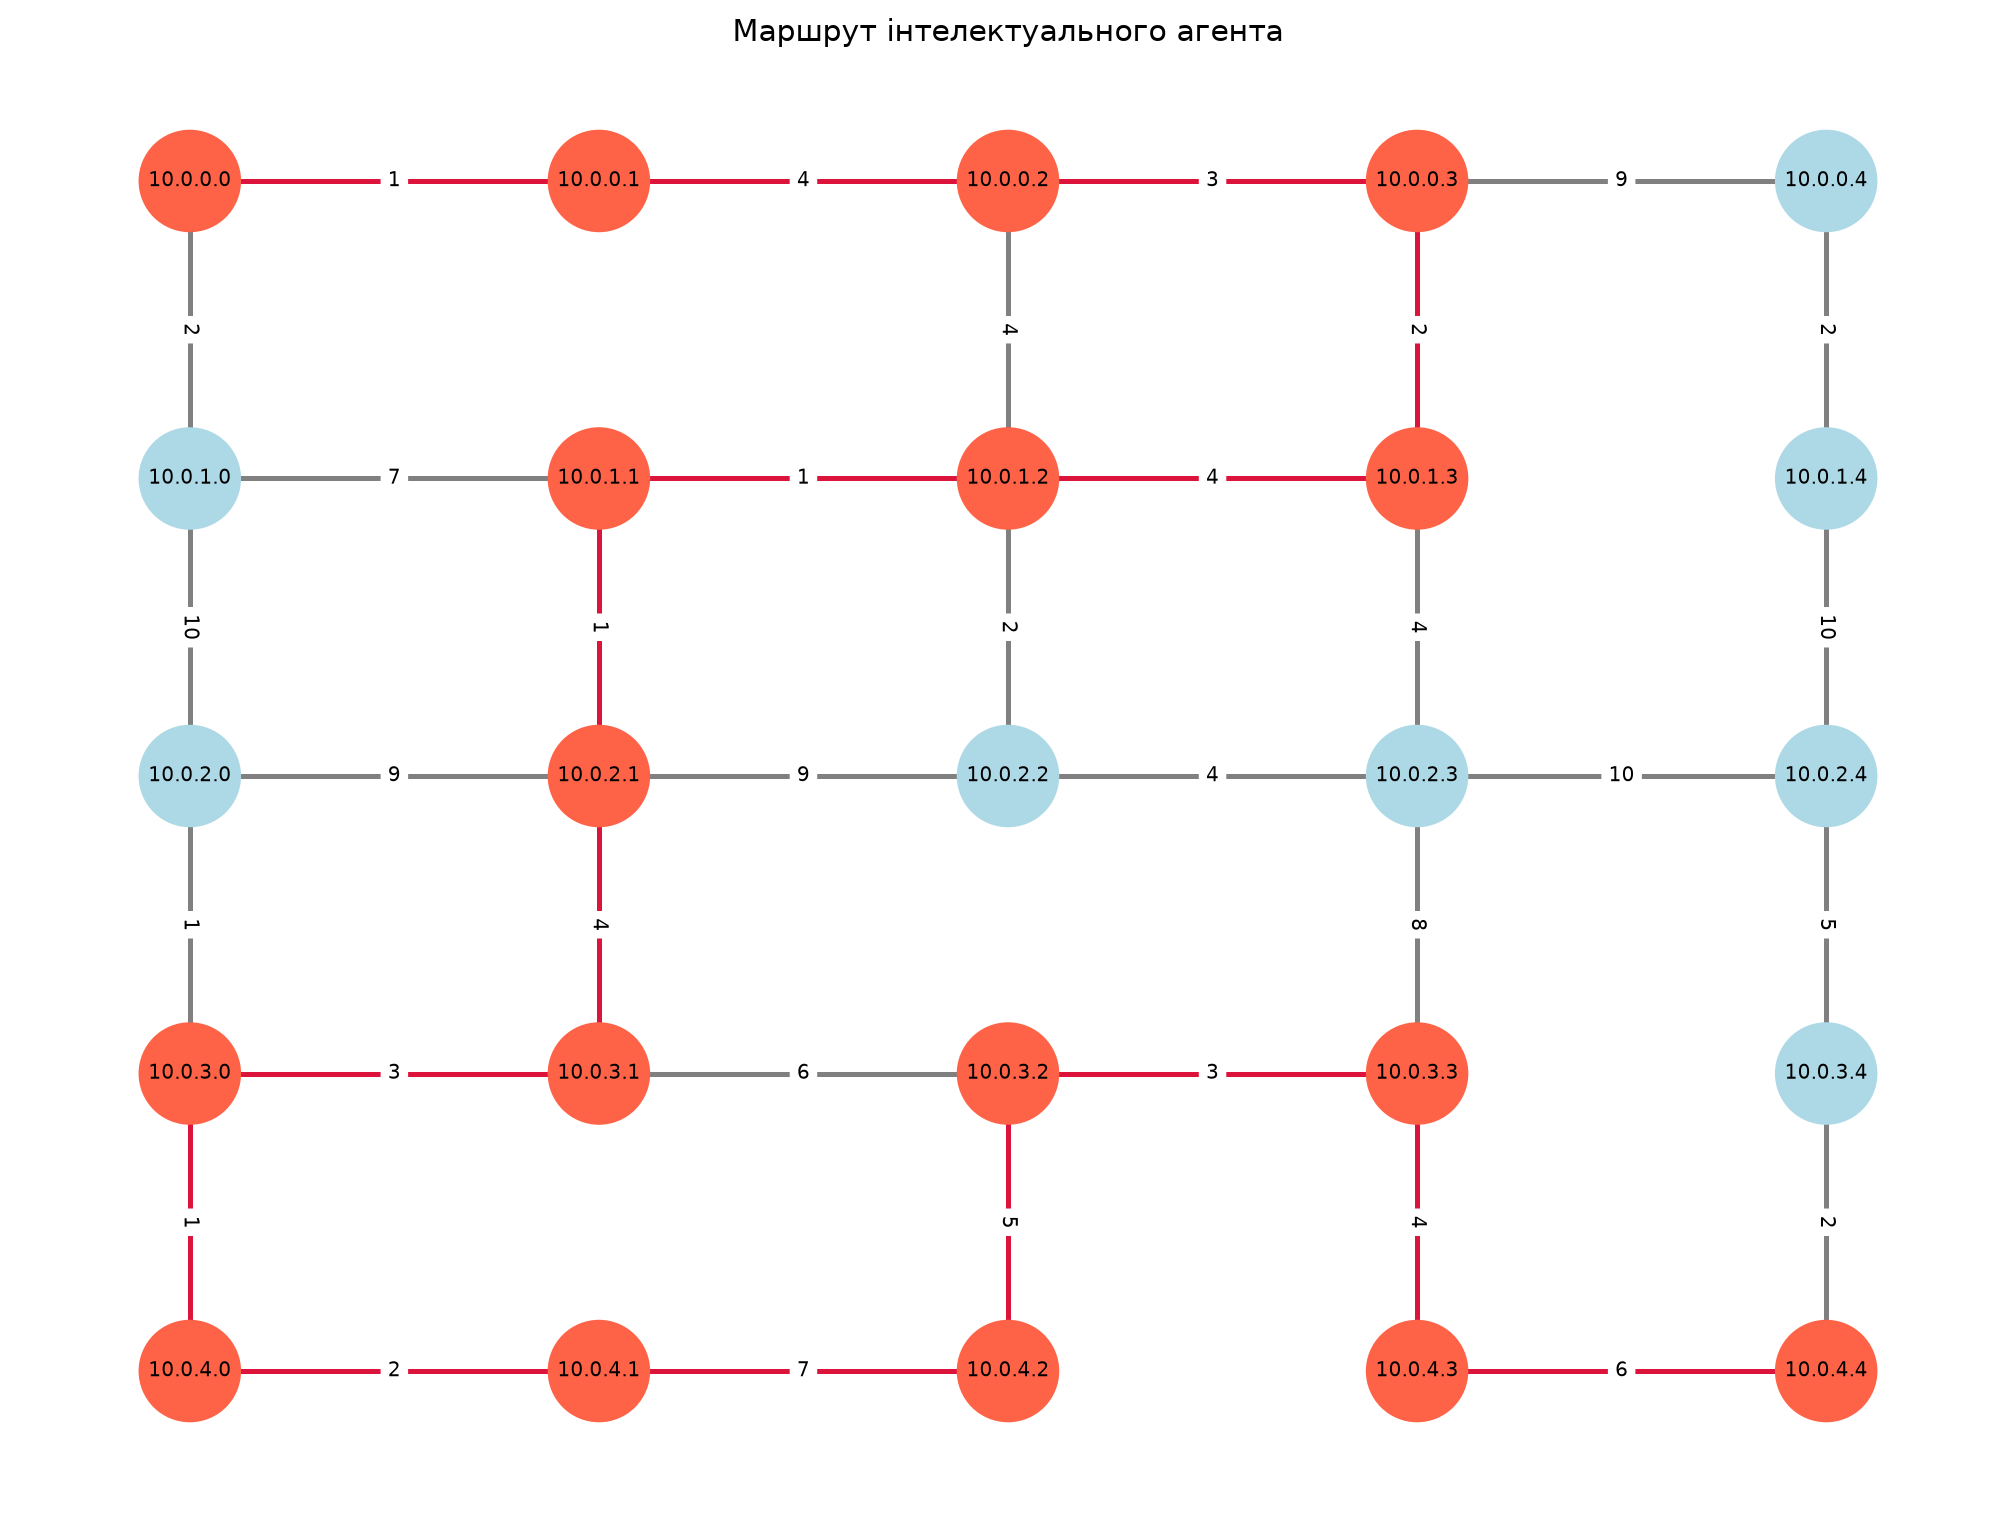
\includegraphics[width=0.94\textwidth]{figures/agent_path.png}
  \caption{Маршрут, знайдений інтелектуальним агентом}
\end{figure}

\begin{figure}[H]
  \centering
  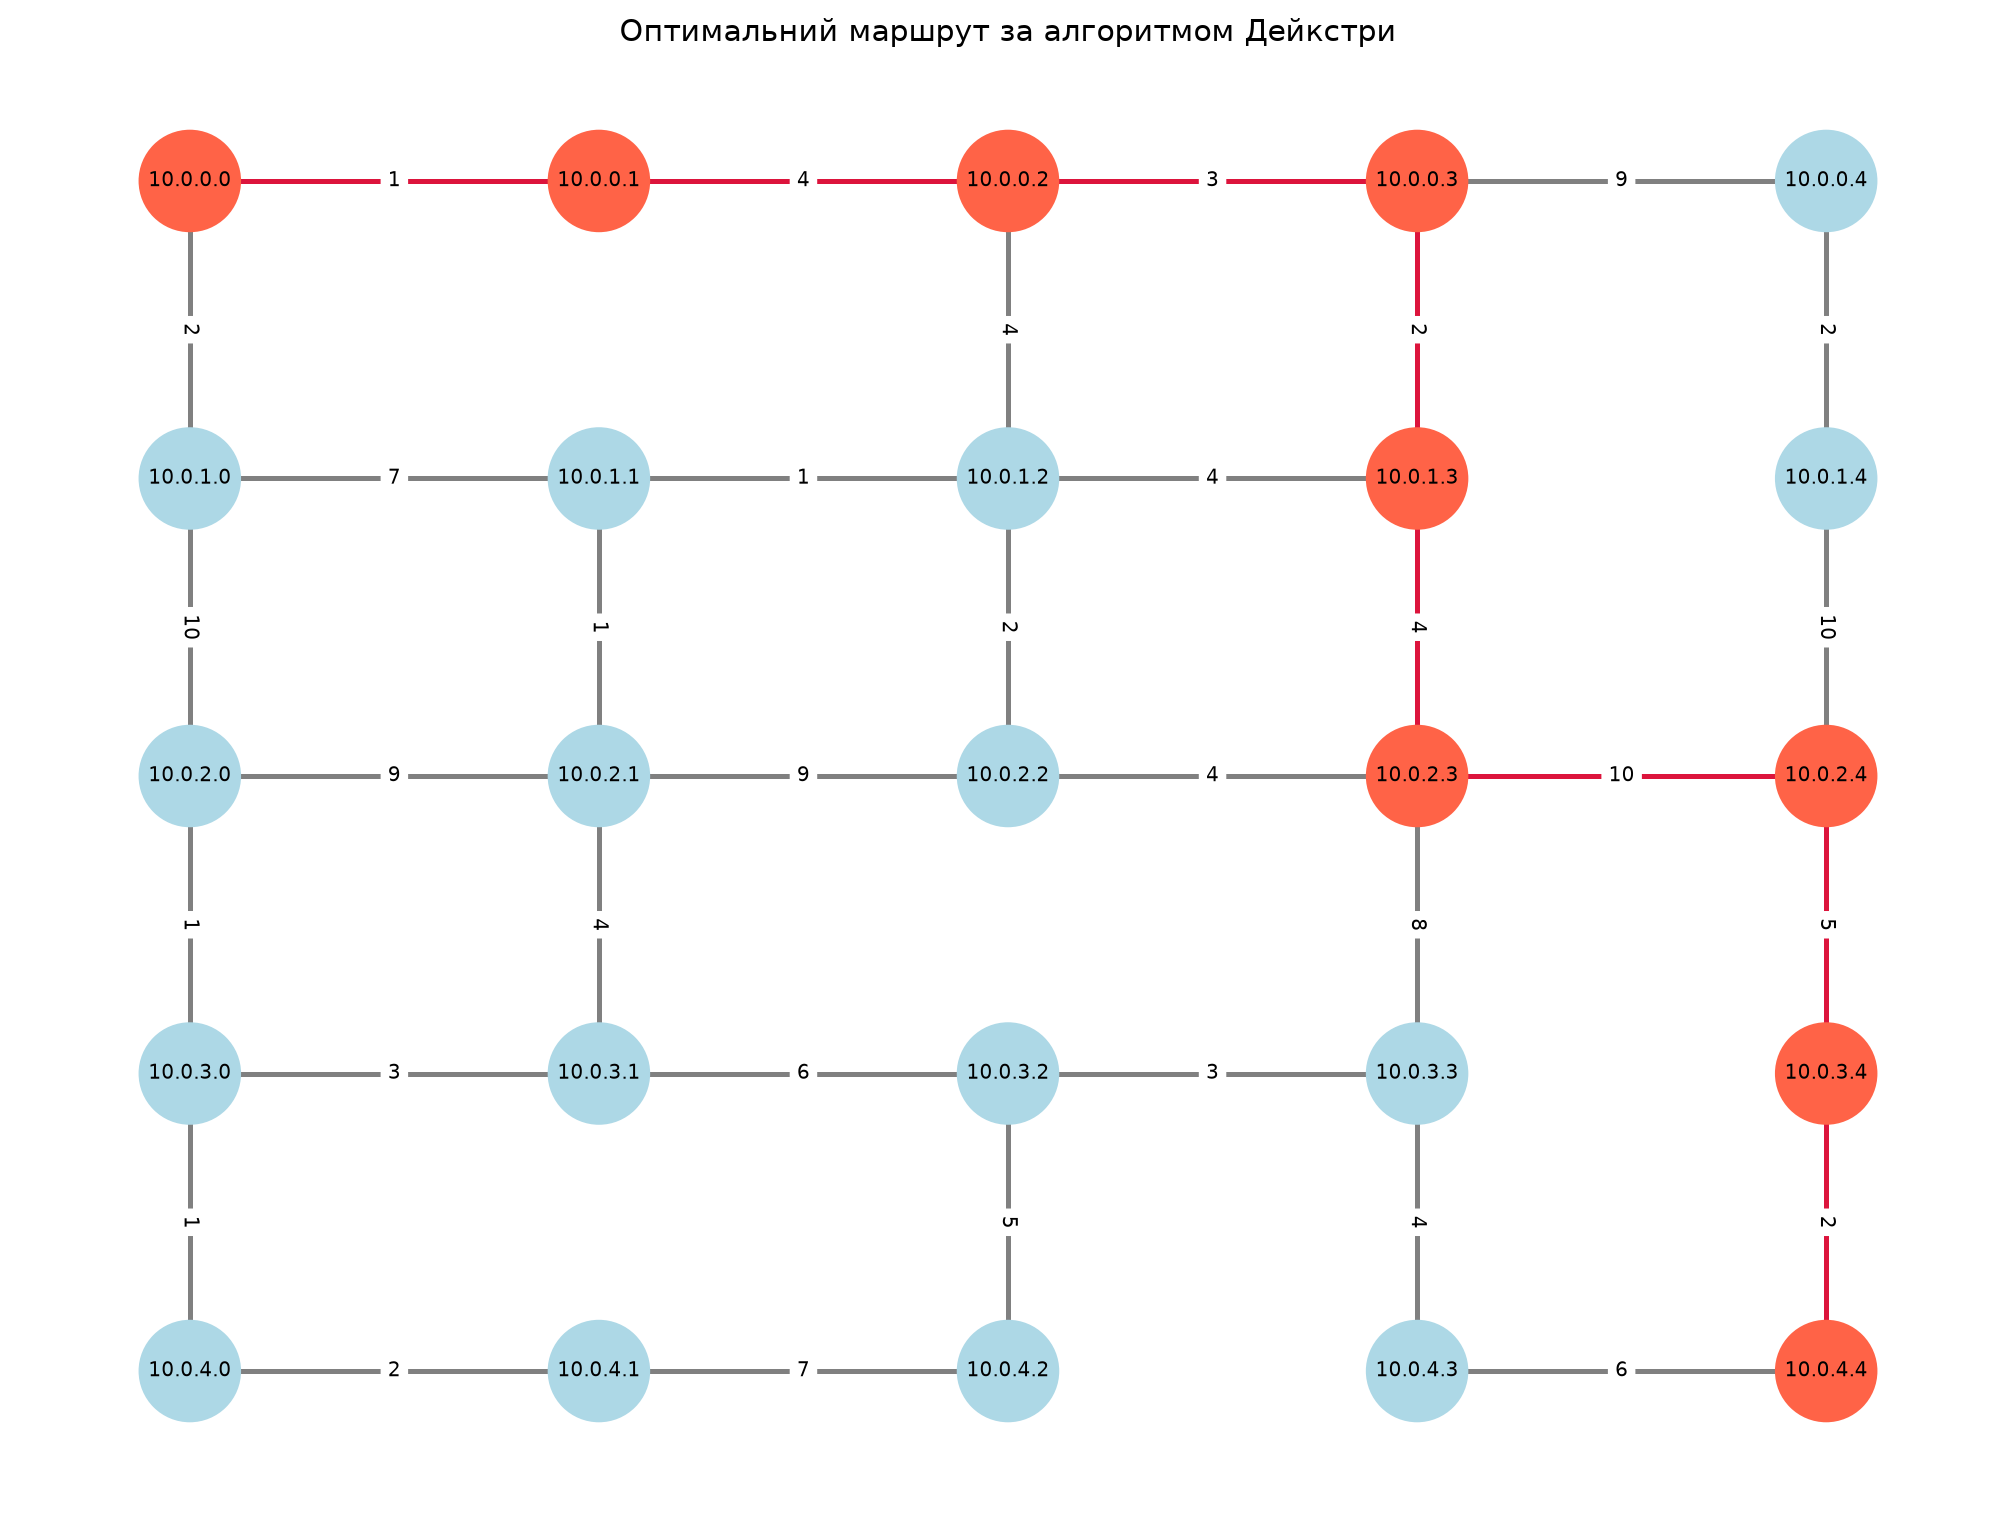
\includegraphics[width=0.94\textwidth]{figures/dijkstra_path.png}
  \caption{Оптимальний маршрут за алгоритмом Дейкстри}
\end{figure}

Для додаткової перевірки виконано три експерименти з різними топологіями.

\begin{table}[H]
\centering
\small
\resizebox{\textwidth}{!}{%
\begin{tabular}{c r r r r}
\toprule
№ & Затримка агента, мс & Затримка Дейкстри, мс & Кількість вузлів агента & Відкликані правила\\
\midrule
1 & 90 & 40 & 21 & 1\\
2 & 50 & 38 & 13 & 0\\
3 & 76 & 35 & 19 & 3\\
\bottomrule
\end{tabular}
}
\caption{Порівняння маршрутів агента та Дейкстри}
\end{table}

У всіх трьох експериментах агент досягнув кінцевого вузла. Водночас його
маршрут не був оптимальним за сумарною затримкою. Це пояснюється тим, що агент
вибирає напрямок за локальною інформацією та не знає вартості продовження
маршруту через ще не досліджені вузли.

\enlargethispage{3\baselineskip}
\section{Висновки}

У лабораторній роботі розроблено інтелектуального агента-мережевого
контролера, який будує маршрут у зваженому графі з обмеженою видимістю.
Агент вибирає невідвіданого сусіда з найменшою локальною вагою, а у випадку
тупика відкликає останнє правило та повертається до попереднього вузла.

Результати показали, що агент успішно досягає отримувача, але локально
жадібний вибір не гарантує глобально найменшої затримки. Алгоритм Дейкстри,
маючи повну топологію, використовується як еталон для порівняння, а різниця
між маршрутами пояснюється обмеженістю інформації агента.

\end{document}
